\documentclass[12pt]{exam}
\usepackage{amsmath}
\usepackage{amssymb}
\usepackage{graphicx}
\usepackage{enumitem}
\usepackage{amsfonts}
\usepackage{amssymb}
\usepackage{ifthen}
\usepackage{geometry}
\noprintanswers

\usepackage{tikz}
\usetikzlibrary{shapes,backgrounds}

\usepackage{framed}

\addtolength{\textheight}{6cm}
\addtolength{\topmargin}{-2cm}
\addtolength{\textwidth}{3cm}
\addtolength{\oddsidemargin}{-1.5cm}
\addtolength{\evensidemargin}{-1.5cm}
\setlength\parindent{0pt}

\newcommand {\DS} [1] {${\displaystyle #1}$}
\newcommand{\vv}{\vspace{.1cm}}

\newcommand{\R}{\mathbb{R}}
\newcommand{\Q}{\mathbb{Q}}
\newcommand{\Z}{\mathbb{Z}}
\newcommand{\N}{\mathbb{N}}

\pagestyle{empty}

\graphicspath{ {./} }

%============================================
%137 COLOUR PALETTE
%============================================

\definecolor{137cp1}{RGB}{13, 33, 161}
\definecolor{137cp2}{RGB}{51, 161, 253}
\definecolor{137cp3}{RGB}{255, 67, 101}
\definecolor{137cp4}{RGB}{232, 144, 5}


%============================================
%HYPERLINKS
%============================================

\usepackage{hyperref}
\hypersetup{colorlinks}
\hypersetup{urlcolor=137cp3, linkcolor=137cp1}

%============================================
%Commands used only for this file
%============================================

\DeclareMathOperator{\arccot}{arccot}

%%%%%%%%%%%%%%%%%%%%%%%%%%%%%%%%%%%%%%%%%


\begin{document}

{\large
	\begin{center}
		{\bf MAT 137Y: Calculus with proofs}\\
		{\bf Assignment 4} \\
		{\bf Due on Thursday, November 26 by 11:59pm via Crowdmark}
	\end{center}
}

\vv

\begin{quotation}
{\bf Instructions:}
	\begin{itemize}
		\item	 You will need to submit your solutions electronically via Crowdmark.   \href{https://www.math.toronto.edu/~alfonso/137/PS/137_CM.html}{See MAT137 Crowdmark help page for instructions}.  Make sure you understand how to submit and that you try the system ahead of time.  If you leave it for the last minute and you run into technical problems, you will be late.  There are no extensions for any reason.
		\item You may submit individually or as a team of two students.  See the link above for more details.
		\item  You will need to submit your answer to each question separately.
		\item  This problem set is about Unit 4.
	\end{itemize}
\end{quotation}
\vv

\begin{enumerate}

\item In this problem, we will only work with functions with domain $\mathbb{R}$ and codomain $\R$.   Therefore, if we say that two functions $f$ and $g$ are equal ($f=g$), it means that 
	$$
		\forall x \in \R, \; f(x)  = g(x) .
	$$
We need a new definition.  We say that a function $f$ is \emph{faithful} when
	\begin{equation*}
		``\mbox{For every two functions } g \mbox{ and } h, \quad f \circ g = f \circ h \implies g = h."
	\end{equation*}
	\begin{enumerate}
		\item  Prove that if a function is one-to-one, then it is faithful.
		
{
	\vv

	\emph{Proof:}

	\vv

	Let's define functions $g$ and $h$ with domain $\R$ and codomain $\R$. Let's define function $f$ as a one to one function.

	\emph{WTS:} $\mbox{For every two functions } g \mbox{ and } h, \quad f \circ g = f \circ h \implies g = h.$


	Assume that $f \circ g = f \circ h$, 
	we can imply that $\forall x \in \R, f(g(x)) = f(h(x)) $.

	Because $f(x)$ is a one-to-one function, we can write that $\forall x_1, x_2 \in \R, f(x_1) = f(x_2) \implies x_1 = x_2$.


	Combining these two, we get:
	$\forall x \in \R, f(g(x)) = f(h(x)) \implies g(x) = h(x)$, which is what we want to show. $\qquad \blacksquare$
}
		
		\item  Prove that if a function is NOT one-to-one, then it is NOT faithful.
{
	\vv

	\emph{Proof:}

	\vv

	Let's define functions $g$ and $h$ with domain $\R$ and codomain $\R$. Let's define function $f$ as an NOT one to one function.

	\emph{WTS:} $\mbox{There exist two functions } g \mbox{ and } h, \quad f \circ g = f \circ h \land g \neq h$

	Because $f(x)$ is not a one-to-one function, we can write that $\exists x_1, x_2 \in \R, f(x_1) = f(x_2) \land x_1 \neq x_2$.
	Take such $x_1, x_2 \in \R$ that satisfy $x_1 \neq x_2, f(x_1) = f(x_2)$.


	Since $g$ and $h$ are functions with domain $\R$ and codomain $\R$, $\exists g, h, S.T. \quad \forall x \in \R, g(x) = x_1 \mbox{ and } h(x) = x_2$.
	Take such $g$ and $h$. Then, $g \neq h$ because $\exists y \in \R, g(y) \neq h(y)$ and $\forall x \in \R, f(g(x)) = f(h(x))$.


	Combining, we can get $\exists g, h, (\forall x \in \R, f(g(x)) = f(h(x))) \land (\exists y \in \R,~ g(y) \neq h(y))$, which is what we want to show. $\qquad \blacksquare$ 
}
	\end{enumerate}

\vv

\newpage

\item   Given two functions $f$ and $g$, we say that $g$ is a \emph{quasi-inverse} of $f$ when
	\begin{quote}
	``There exists a non-empty, open interval $I$ contained in the domain of $f$, such that the restriction of $f$ to $I$ is one-to-one, and $g$ is the inverse of that restriction."
	\end{quote}
For example, $\arctan$ is a quasi-inverse of $\tan$.

Construct a function $f$ that satisfies all the following properties at once:
	\begin{enumerate}
		\item  The domain of $f$ is $\R$.
		\item  $f$ is differentiable.
		\item  \label{long} For every $c>0$ there exists a quasi-inverse $g$ of $f$ such that $g$ is differentiable at $0$ and and $0 < g'(0) < c$.
	\end{enumerate}

We want an explicit equation for $f$ and a graph (feel free to use Desmos, for example).  Once you have the function, you may use the graph to help justify why it satisfies property (c), rather than proving it entirely algebraically.  Use your judgement to decide how much of an explanation you need.

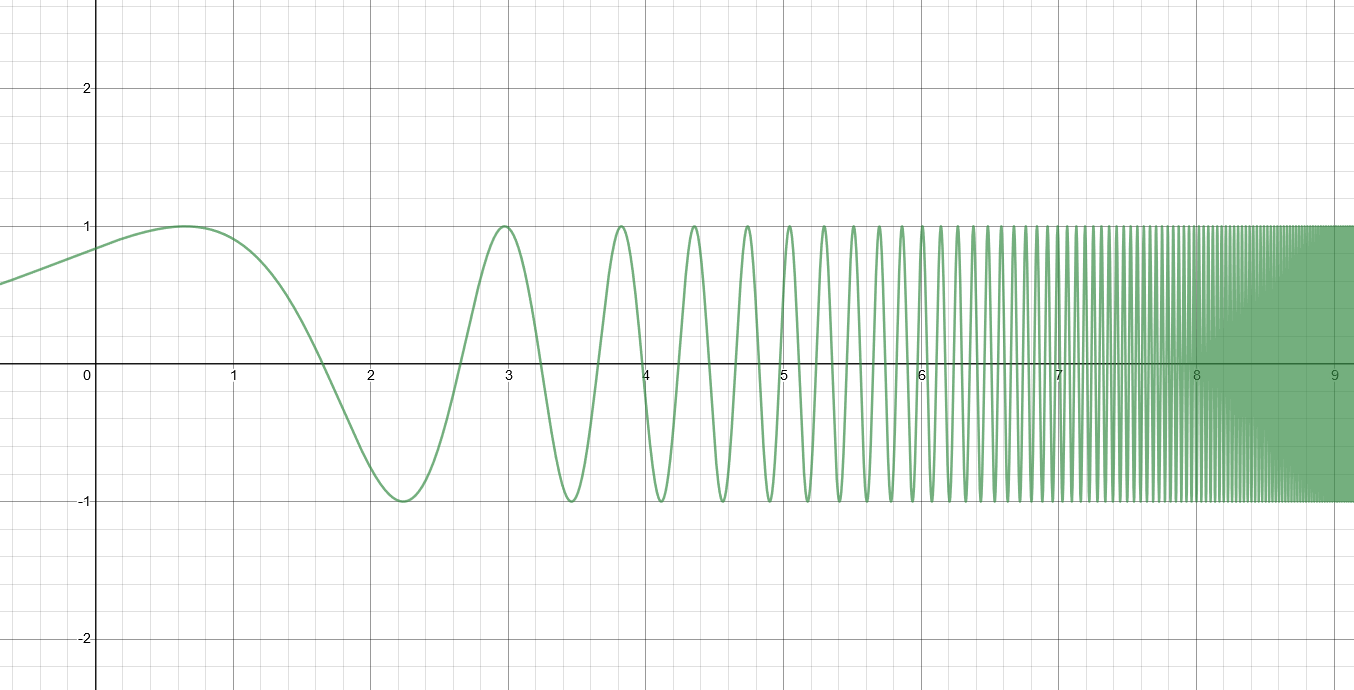
\includegraphics[scale=0.4]{a4}


We want to define function $f$ as $\sin(2^x)$ of $f$.

The domain of $f(x)=\sin(2^x)$ is $x\in\R.$

Since we know $\sin(x) \land 2^x$ are both differentiable, $\frac{d}{dx}[f(x)]=\frac{d}{dx}[\sin(2^x)]$, by using the Chain Rule:
\begin{align*}
    \frac{d}{dx}[f(x)]&=\frac{d}{dx}[\sin(2^x)]\\
    f'(x)&=\cos(2^x)\cdot(2^x)'\quad(\frac{d}{dx}[\sin(x)]=\cos(x))\\
    f'(x)&=\cos(2^x)\cdot[2^x\cdot\ln(2)]\quad(\frac{d}{dx}[a^x]=a^x\cdot\ln(a))\\
    f'(x)&=2^x\ln(2)\cos(2^x)
\end{align*}

For the property(c), let $c>0.$

When $f$ is increasing or decreasing on a specific interval we know this interval is one-to-one.

Since we want to find $g \mbox{ which is } \emph{quasi-inverse}$ of $f$. By using theorem of derivative of the inverse of a function $(f^{-1})'(f(x)) = \frac{1}{f'(x)}$, we know $g'(0)=\frac{1}{f'(x)}$ and $f(x)=0.$ From $f(x)=\sin(2^x)$ and $0<g'(0)<c,$ we know that $g'(0)=\frac{1}{f'(x)}=\frac{1}{2^x\ln(2)\cos(2^x)}<c.$
\begin{align*}
    \frac{1}{2^x\ln(2)\cos(2^x)}&<c\\
    \frac{1}{2^x\ln(2)}&<c\quad(\sin(2^x)=0\implies\cos(2^x)=1)\\
    \frac{1}{2^x}&<c\ln(2)\quad(\ln(2)>0)\\
    2^x&>\frac{1}{c\ln(2)}\quad(2^x>0\mbox{ and }c\ln(2)>0)\\
    \log_2(2^x)&>\log_2(\frac{1}{c\ln(2)})\quad(x_1>x_2\iff \log x_1>\log x_2)\\
    x&>\log_2(\frac{1}{c\ln(2)})
\end{align*}

So by graph we take $x>\log_2(\frac{1}{c\ln(2)})$, and we look at the right of this point to choose the interval $I$ where $f$ is increasing or decreasing and $\exists a\in I$ such that $f(a)=0$. Then we find $g(x)$ as \emph{quasi-inverse} of $f$ is $\log_2(\arcsin(x)).$

Since $\forall x\in\R, \frac{1}{2^x\ln(2)\cos(2^x)}=\frac{1}{2^x\ln(2)}>0\quad(2^x>0)$, We have proven $g$ is differentiable at 0 and $0 < g'(0) < c$.

\vv

\item  In the videos we discussed how to define the number $e$, how to define exponentials and logarithms, and how to obtain formulas for their derivatives.      In this problem you are going to get the same formulas in a different way.

We will assume that exponentials and logarithms are well-defined and continuous, and we will assume the common properties of exponentials and logarithms.   However, we assume we still do not know anything about their derivatives -- that is the point of this problem!

For this problem we will define the number $e$ as this limit\footnote{If you learned a definition of the number $e$ in high-school, it was probably this one.}
	\begin{equation}  \label{eq:e}
		e = \lim_{x \to 0} \left( 1 + x \right)^{1/x}.
	\end{equation}
We should first prove that this limit exists, but we are going to skip that part.  Let's just assume the limit exists and therefore this is a valid way to define the number $e$.
  Other than that, during this problem, make a particular effort to explain what you are doing: specifically mention any property, result, or identity that you use in any step.

	\begin{enumerate}
		\item  Prove that \DS{\lim_{x \to 0} \frac{\ln (1+x)}{x} = 1}.
		
			\emph{Hint:}  Use Equation \eqref{eq:e} and a result from Video 2.16.
		\vv
		
        \emph{Proof:}
        
        \vv
        
        Since we assume that exponentials and logarithms are well-defined and continuous. We suppose function $g=\ln(x)$, then $g$ is continuous at $e$.
        
        Since we assume $\lim_{x \to 0} \left( 1 + x \right)^{1/x}$ exists and define it as the number $e$, by using Theorem 3 in Video 2.16,
        
        $$
            \lim_{x \to a}f(x)=L \land {g\ \mbox{is continuous at}\ L} \implies \lim_{x \to a}g[f(x)]=g(L)
        $$
        
        We suppose $f(x)=\left( 1 + x \right)^{1/x}$, $a=0$ and $L=e$, then we can get,
        
        $$
            \lim_{x \to 0} g[\left( 1 + x \right)^{1/x}]=g(e)=\ln(e)=1
        $$
        
        We also know that,
        
        $$
            \lim_{x \to 0} g[\left( 1 + x \right)^{1/x}]=\lim_{x \to 0} \ln[\left( 1 + x \right)^{1/x}]=\lim_{x \to 0} [\frac{1}{x}\cdot\ln(1 + x)]=\lim_{x \to 0}\frac{\ln (1+x)}{x}
        $$
        
        We have proven that \DS{\lim_{x \to 0} \frac{\ln (1+x)}{x} = 1} as needed. $\qquad \blacksquare$
		\item  Consider the function $L(x) = \ln x$.  Prove that $L$ is differentiable everywhere on its domain, and find a formula for its derivative.
			
			\emph{Hint:}  Use the definition of derivative as a limit.  While any of the two ``versions" works, we recommend you use the version ``as $h \to 0$".  Then use the properties of logarithms.
		\vv
		
		\emph{Proof:}
		
		\vv
		
		First we need to state the domain of $L(x)=\ln(x)$ is $x\in(0,\infty).$
		To investigate the differentiability of $L(x)$, we consider \DS{\lim_{h \to 0} \frac{L(x+h)-L(x)}{h}.} Assume $L(x)=\ln(x).$ Note that:
		\begin{align*}
		    \lim_{h \to 0} \frac{L(x+h)-L(x)}{h}&=\lim_{h \to 0} \frac{\ln(x+h)-\ln(x)}{h}\\
		    &=\lim_{h \to 0} \frac{\ln(\frac{x+h}{x})}{h}\quad(x\neq0 \land \ln(a)-\ln(b)=\ln(\frac{a}{b}))\\
		    &=\lim_{h \to 0} \frac{\ln(1+\frac{h}{x})}{h}\\
		    &=\lim_{h \to 0}[ \frac{\ln(1+\frac{h}{x})}{\frac{h}{x}}\cdot\frac{1}{x}]\quad(x\neq0)\\
		    &=\lim_{m \to 0}[ \frac{\ln(1+m)}{m}\cdot\frac{1}{x}]\quad(\mbox{set } m=\frac{h}{x})\\
		    &=\lim_{m \to 0} \frac{\ln(1+m)}{m}\cdot\lim_{m \to 0}\frac{1}{x}\quad(\mbox{Limit Laws})\\
		    &=1\cdot\lim_{m \to 0}\frac{1}{x}\quad(\lim_{x \to 0} \frac{\ln (1+x)}{x} = 1 \mbox{ from Q3a})\\
		    &=\frac{1}{x}
		\end{align*}
		Since $\frac{1}{x}$ always exists given $x\in(0,\infty)$, we have shown $L$ is differentiable everywhere on its domain $x>0$, and find a formula $\frac{1}{x}$ for its derivative.$\quad\blacksquare$
		
		\item  Consider the function \DS{E(x) = e^x}.  Using the fact that $E$ and $L$ are inverses of each other, and now that you have a formula for $L'$, obtain a formula for $E'$.
		
			\emph{Note:}  This is similar to what you learned in the videos, but in the videos we used a formula for $E'$ to obtain a formula for $L'$.
	    \vv
	    
	    \emph{Proof:}
	    
	    \vv
	    
	    Since $E$ and $L$ are inverses of each other, we can get $L(E(x))=x.$ The domain of $E(x)$ is $x\in\R.$ The domain of $L(x)$ is $x > 0.$ Assume $E(x)=e^x>0,\mbox{ then } E(x)\neq0 \land E(x)\mbox{ is in the domain of } L(x).$
	    
	    By implicit differentiation of $L(E(x))=x$, 
	    \begin{align*}
	        L'(E(x))\cdot E'(x)&=1\quad(\mbox{Chain Rule})\\
	        \frac{1}{E(x)}\cdot E'(x)&=1\quad(E(x)\neq0 \land L'(x)=\frac{1}{x}\mbox{ from Q3b})\\
	        E'(x)&=E(x)=e^x
	    \end{align*}
	    We have proven $E'(x)=e^x$ as needed. $\quad\blacksquare$
	\end{enumerate}

\vv

\item  We define $\arccot$ as the inverse function of the restriction of $\cot$ to \DS{(0, \pi)}.
	\begin{enumerate}
		\item \emph{[Do not submit]}  Sketch a graph of $\cot$ and convince yourself that this is the most reasonable choice to define $\arccot$.
		\item   Obtain and prove a formula for \DS{\frac{d}{dx} \arccot x}.
		
			\emph{Hint:}  Imitate the proof in Video 4.13.
		
		\vv
		
		\emph{Proof:}
		
		\vv
		
		We set the domain of $\cot x$ as $x\in(0,\pi).$ Then domain of $\arctan x$ is $x\in(-\infty,\infty).$ Since $\cot x$ and $\arccot x$ are inverse functions, we can get $\cot(\arccot x)=x.$
		
		We set the formula $\theta=\arccot{x}$. The range of $\theta \mbox{ is } (0, \pi)$. We can also get $\cot\theta=x$.
		
		Then we find the derivative of $\cot x$ is
		\begin{align*}
		    \frac{d}{dx}[\cot x]&=\frac{d}{dx}[\frac{\cos x}{\sin x}]\\
		    &=\frac{(\cos x)'\cdot\sin x-(\sin x)'\cdot\cos x}{(\sin x)^2}\quad(\mbox{Quotient Rule})\\
		    &=-\frac{(\sin x)^2+(\cos x)^2}{(\sin x)^2}\quad((\cos x)'=-\sin x \land (\sin x)'=\cos x)\\
		    &=-\frac{1}{(\sin x)^2}\quad((\sin x)^2+(\cos x)^2=1)\\
		    &=-\csc^2 x
		\end{align*}
		By implicit differentiation of $\cot(\arccot x)=x,$
		\begin{align*}
		    \frac{d}{dx}[\cot(\arccot x)]&=\frac{d}{dx}[x]\\
		    [\cot(\arccot x)]'\cdot (\arccot x)'&=1\quad(\mbox{Chain Rule})\\
		    [\cot(\theta)]'\cdot (\arccot x)'&=1\quad(\theta=\arccot{x})\\
		    -\csc^2\theta\cdot(\arccot x)'&=1\quad(\frac{d}{dx}[\cot x]=-\csc^2 x)\\
		    -(1+x^2)\cdot(\arccot x)'&=1\quad(\csc^2\theta=\frac{\sin^2\theta+\cos^2\theta}{\sin^2\theta}=1+\cot^2\theta=1+x^2)(\cot\theta=\frac{\cos\theta}{\sin\theta}=x)\\
		    (\arccot x)'&=-\frac{1}{1+x^2}
		\end{align*}
		We have proven $\frac{d}{dx} \arccot x=-\frac{1}{1+x^2}$ as needed. $\quad\blacksquare$
		
		\item The following ``theorem" is not quite true as stated:
		
			\begin{quotation}
			{\bf Flawed ``Theorem":}   \DS{ \arccot x \; = \; \arctan \frac{1}{x} }
			
			{\bf Fake ``Proof":}   \vspace{-.5cm}
				\begin{align*}
					\theta \; =& \; \arccot x \\
					 \cot \theta \; =& \;  x \\
					 \tan \theta \; = \; \frac{1}{\cot \theta} \; =& \; \frac{1}{x} \\
					 \theta  \; =& \;  \arctan \frac{1}{x}  
				\end{align*}
				\ \hfill $\square$
			\end{quotation}

	Explain the problem with the statement of the theorem and the errors in the proof.  Then fix them: correct the statement, and write a correct proof.
	
	\vv
	
	\emph{Problem:}
	
	\vv
	
	This Flawed 'Theorem' didn't give any domain of $x$, in this theorem we can clearly see $\frac{1}{x}$, so $x$ cannot be 0. So the writer needs to discuss this theorem by cases. In the proof, it also didn't have any domain of $x$ or any range of $\theta.$ So we need to have cases discussion in the proof.
	
	\vv
	
	\emph{Theorem:}
	
	\vv
	$$
	\begin{cases}
	    x\in(-\infty, 0),&\arccot x=\pi+\arctan\frac{1}{x}\\
	    x=0,&\arctan\frac{1}{x} \mbox{ is not defined}\\
	    x\in(0, \infty),&\arccot x=\arctan\frac{1}{x}\\
	\end{cases}
	$$
	\vv
	
	\emph{Proof:}
	
	\vv
	
	Case 1: When $x\in(-\infty, 0)$, assume $\theta=\arctan x \land \theta \in(\frac{\pi}{2},\pi).$ Since $\arccot x$ and $\cot x$ are inverse functions,
	\begin{align*}
	    \cot\theta&=x\\
	    \cot(\theta-\pi)&=x\quad(\cot x\mbox{ has period of }\pi)\\
	    \tan(\theta-\pi)=\frac{1}{\cot(\theta-\pi)}&=\frac{1}{x}\quad(\cot\theta=x\land x\neq0)\\
	    \arctan(\tan(\theta-\pi))&=\arctan(\frac{1}{x})\\
	    \theta-\pi&=\arctan(\frac{1}{x})\quad(\mbox{Inverse Function})\\
	    \theta&=\pi+\arctan(\frac{1}{x})\quad(\arctan(\frac{1}{x})\in(-\frac{\pi}{2},0))\\
	    \arctan x&=\pi+\arctan(\frac{1}{x})\quad(\arctan x=\theta)
	\end{align*}
	We add $\pi$ to $\arctan(\frac{1}{x})$ since we need to have the same domain for $\theta$.\\
	
	Case 2: When $x=0,\arctan\frac{1}{x} \mbox{ is not defined since 0 can not be denominator.}$\\
	
	Case 3: When $x\in(0, \infty)$, assume $\theta=\arctan x \land \theta \in(0, \frac{\pi}{2}).$ Since $\arccot x$ and $\cot x$ are inverse functions,
	\begin{align*}
	    \cot\theta&=x\\
	    \tan\theta=\frac{1}{\cot\theta}&=\frac{1}{x}\quad(\cot\theta=x\land x\neq0)\\
	    \arctan(\tan\theta)&=\arctan(\frac{1}{x})\\
	    \theta&=\arctan(\frac{1}{x})\quad(\mbox{Inverse Function} \land \arctan(\frac{1}{x})\in (0, \frac{\pi}{2}))\\
	    \arctan x&=\arctan(\frac{1}{x})\quad(\arctan x=\theta)
	\end{align*}
	We have proven:
	$$
	\begin{cases}
	    x\in(-\infty, 0),&\arccot x=\pi+\arctan\frac{1}{x}\\
	    x=0,&\arctan\frac{1}{x} \mbox{ is not defined}\\
	    x\in(0, \infty),&\arccot x=\arctan\frac{1}{x}\\
	\end{cases}
	$$
	\qquad as needed. $\quad\blacksquare$

	\end{enumerate}


\end{enumerate}
\end{document}

%%%%%%%%%%%%%%%%%%%%%%%%%%%%%%%%%%%%%%%
%%%%%%%%%%%%%%%%%%%%%%%%%%%%%%%%%%%%%%%
%%%%%%%%%%%%%%%%%%%%%%%%%%%%%%%%%%%%%%%

